\begin{figure*}[!htb]
    \centering
    \subfloat[Samples from the cMNIST training set, $\sigma=0$.]{%
        \scalebox{0.3}{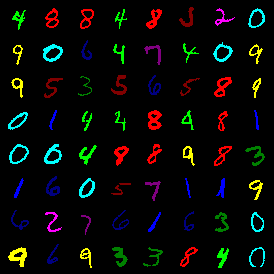
\includegraphics[width=\textwidth]{./Images/cmnist/cflow_original_task_x_scale_0.png}}%
        \label{fig:cflow_cmnist_task_train}
    }
    % \hfill
    % \subfloat[Samples from the cMNIST test set with $\sigma=0.02$.]{%
    %     \scalebox{0.225}{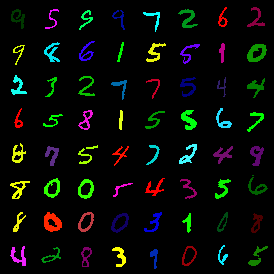
\includegraphics[width=\textwidth]{./Images/cmnist/cflow_pretrain_x.png}}%
    %     \label{fig:cflow_cmnist_pretrain}
    % }
    \hfill
    \subfloat[$x_u$ null-samples from the cFlow model.]{%
        \scalebox{0.3}{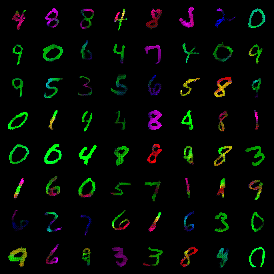
\includegraphics[width=\textwidth]{./Images/cmnist/cflow_task_xy_scale_0.png}}%
        \label{fig:cflow_cmnist_y}
    }
    \hfill
    \subfloat[$x_b$ null-samples from the cFlow model.]{%
        \scalebox{0.3}{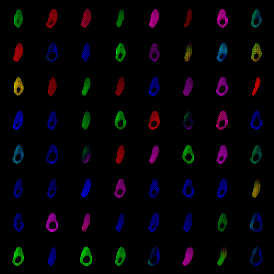
\includegraphics[width=\textwidth]{./Images/cmnist/cflow_task_xs_scale_0.png}}%
        \label{fig:cflow_cmnist_s}
    }
    \caption{
        Sample images from the coloured MNIST dataset problem with $10$ predefined mean colours.
        (a): Images from the spuriously correlated subpopulation where colour is a reliable signal of the digit class-label.
        (b-c): Results of running our approach realised with cFlow on the cMNIST dataset.
        The model learns to retain the shape of the digit shape while removing the relationship with colour.
        A downstream classifier is now less prone to exploiting correlations between colour and the digit label class.
    }\label{fig:cmnist}
\end{figure*}


\section{Background}\label{sec:background}
% \noindent We frame our approach in the context of relevant literature on the interrelated problems of fair representation learning and learning representations free of spurious correlations.
% The background is far too long - we also need to touch on the interpretability literature

% \subsubsection{Learning fair representations.}
\textbf{Learning fair representations.}
%As we have alluded to, the goal of producing invariant representations is similar to that of producing \emph{fair} representations.
% In fairness problems, there is usually a \emph{sensitive attribute}, $s$ (for example, gender or race),
% that should not be used to make decisions.
Given a sensitive attribute $s$ (for example, gender or race) and inputs $\bm{x}$,
a fair representation $\bm{z}$ of $\bm{x}$ is then one for which $\bm{z} \perp s$ holds,
while ideally also being predictive of the class label $y$.
\cite{ZemWuSwePitetal13} was the first to propose the learning of fair representations which allow for transfer to new classification tasks.
More recent methods are often based on variational autoencoders (VAEs)~\cite{kingma2013auto,LouSweLi15,edwardsstorkey,beutel}.
The achieved fairness of the representation can be measured with various fairness metrics.
These measure, however, usually how fair the predictions of a classifier are
and not how fair a representation is.
% defined with respect to predictions and not representations.

% There is not one metric universally best-suited to measuring the invariance (or fairness) of representations.
The appropriate measure of fairness for a given task is domain-specific \cite{liu2018delayed}
and there is often not a universally accepted measure.
However, \emph{Demographic Parity} is the most widely used~\cite{LouSweLi15,edwardsstorkey,beutel}.
Demographic Parity demands $\hat{y} \perp s$ where $\hat{y}$ refers to the predictions of the classifier.
In the context of fair representations, we measure the Demographic Parity of a downstream classifier, $f(\cdot )$, which is trained on the representation $z$ i.e.  $f: Z \to \hat{Y}$.

A core principle of all fairness methods is the \emph{accuracy-fairness trade-off}.
As previously stated, the fair representation should be invariant to $s$ ($\to$ fairness) but still be predictive of $y$ ($\to$ accuracy).
These desiderata cannot, in general, be simultaneously satisfied if $s$ and $y$ are correlated.
% We explore this trade-off with our method as well. % DO WE?!?!?!?!?


The majority of existing methods for fair representations also make use of $y$ labels during training,
in order to ensure that $\bm{z}$ remains predictive of $y$.
This aspect can, in theory, be removed from the methods,
but then there is no guarantee that information about $y$ is preserved \cite{LouSweLi15}. 
% Existing methods designed to create fair representations can, in theory, be extended to the regime in which only the $s$, and not the $y$, labels are available. 
% However, it is not without its drawbacks as, in removing $s$, there is no guarantee that information about $y$ is preserved \cite{LouSweLi15}. 
% For this reason, $y$ is typically supplied during training and the representation encouraged to be predictive of it.

%\subsection{Learning Fair and Transferable Representations}
% \subsubsection{Learning fair representations that are transferable and in the data domain.}
\textbf{Learning fair, transferrable representations.}
% Outside of computer vision, \cite{madras2018learning} have also worked on removing a problematic spurious correlation.
In addition to producing fair representations, \cite{madras2018learning} want to ensure the representations are transferrable.
Here, an adversary is used to remove sensitive information from a representation $z$.
Auxiliary prediction and reconstruction networks, to predict class label $y$
% to ensure it remains predictive of $y$
and reconstruct the input $x$ respectively,
are trained on top of $z$, with $s$ being ancillary input to the reconstruction.
% alongside a reconstruction loss computed with respect to the output of a decoder that takes $z$ and the sensitive label $s$ as input is added. 
% This is so that $x$ can still be reconstructed from $z$, despite the removal of $s$.
%The decoder is utilised only for the purpose of maximum likelihood learning of the data distribution.
% By conditioning the decoder on the sensitive attribute, information about it can be ``off-loaded'' from the encoder such that information about $s$ need not be contained in the fair representation while still permitting the use of a reconstruction loss needed to capture non-sensitive information.
% The decoder plays a role only in the loss function.
% In contrast, we make explicit use of the decoder not only for characterising the behaviour of the model and also for evaluation.

Also related is \cite{creager2019flexibly} who employ a FactorVAE \cite{kim2018disentangling} regularised for fairness.
The idea is to learn a representation that is both disentangled and invariant to multiple sensitive attributes.
This factorisation makes the latent space easily manipulable such that the different subspaces can be freely removed and composed at test time.
Zeroing out the dimensions or replacing them with independent noise imparts invariance to the corresponding sensitive attribute.
This method closely resembles ours when we use an invertible encoder.
However, the emphasis of our approach is on interpretability, information-preservation, and coping with sampling bias - especially extreme cases where $|\, \textrm{supp}(S_{tr} \times Y_{tr}) | < |\, \textrm{supp}(S_{te} \times Y_{te}) |$.
% Namely, the invertibility of the network means we can optimise for invariance singularly without the burden of a reconstruction loss.
% While we do not explicitly consider the case of multi-attribute fairness, our method can be easily adapted for this use-case.

Attempts were made by \cite{QuaShaTho19} prior to this work to learn fair representations in the data domain in order to make it interpretable and transferable.
In their work, the input is assumed to be additively decomposable in the feature space into a \emph{fair} and \emph{unfair} component, which together can be used by the decoder to recover the original input.
This allows us to examine representations in a human-interpretable space and confirm that the model is not learning a relationship reliant on a sensitive attribute.
Though a first step in this direction, we believe such a linear decomposition is not sufficiently expressive to fully capture the relationship between the sensitive and non-sensitive attributes.
Our approach allows for the modelling of more complex relationships.

% \subsubsection{Learning in the presence of spurious correlations.}
\textbf{Learning in the presence of spurious correlations.}
% As  previously  discussed,  the  goal  of  producing  fair representations is similar to the goal of producing representations invariant to spurious correlations found in the training data.
Strong spurious correlations make the task of learning a robust classifier challenging: the classifier may learn to exploit correlations unrelated to the true causal relationship between the features and label, and thereby fail to generalise to novel settings.
This problem was recently tackled by \cite{ln2l} who apply a penalty based on the mutual information between the feature embedding and the spurious variable. 
While the method is effective under mild biasing, we show experimentally that it is not robust to the range of settings we consider.

Jacobsen et al. \cite{JacBehZemBet19} explore the vulnerability of traditional neural networks to spurious variables -- e.g., textures, in the case of ImageNet \cite{Geir18} -- and propose a INN-based solution akin to ours.
The INN's encoding is split such that one partition, $z_b$ is encouraged to be predictive of the spurious variable while the other serves as the logits for classification of the semantic label. 
Information related to the nuisance variable is ``pulled out'' of the logits as a result of maximising $\log p(s|z_n)$.
This specific approach, however, is incompatible with the settings we consider, due to its requirement that both $s$ and $y$ be available at training time.

Viewing the problem from a causal perspective, \cite{arjovsky2019invariant} develop a variant of empirical risk minimisation called invariant risk minimisation (IRM).
The goal of IRM is to train a predictor that generalises across a large set of unseen environments; because variables with spurious correlations do not represent a stable causal mechanism, the predictor learns to be invariant to them. IRM assumes that the training data is not \emph{iid} but is partitioned into distinct environments, $e \in E$. The optimal predictor is then defined as the minimiser of the sum of the empirical risk $R_e$ over this set. In contrast, we assume possession of only a single source of \emph{labelled}, albeit spuriously-correlated, data, but that we have a second source of data that is free of spurious correlations, with the benefit being that it only needs to be labelled \emph{with respect to $s$}.

% The model thereby enforces their independence.
% This is achieved with an adversarial approach, borrowing the gradient reversal technique from \cite{ganin2016domain}.
%The authors construct the coloured MNIST dataset in two steps.
%First, ten distinct colours are assigned to each digit uniquely; these colours parameterise the means of ten corresponding Gaussian distributions from which colour samples are drawn.
%The standard deviation ($\sigma$) of the Gaussian distribution controls the dispersion of the sampled colours around these means.
% To demonstrate the effectiveness of their model, \cite{ln2l} construct a coloured version of the MNIST dataset as follows.
% During training, colours are sampled from a Gaussian distribution (with standard deviation $\sigma$) where each digit is associated with a single fixed mean colour.
%the colours are sampled abiding by this one-to-one colour mapping;
% At test time however, a colour mean is chosen at random from the 10 mean colours used during training.
% The actual colour is sampled with the same $\sigma$ as in the training set.
%there is no such designation and colours are sampled randomly and unrestrictedly from the complete palette.
%As such, a classifier that lazily minimises its loss by treating the pixel values as a lookup table falls flat at inference owing to a shift in the distribution of the spurious variables away from that of the target's.
% We follow this approach to evaluate performance of our NoSiNN framework in a synthetic setting (see Fig. \ref{fig:cmnist} for qualitative results).

% For the training strategy of the \cite{ln2l} model, a neural network is trained to predict the digit class, $y$, while an adversarial network takes one of the intermediate layers as input to predict the spurious value, colour.
% The first network seeks to prevent the adversary from making correct predictions, which means discarding or obfuscating information about colour.
% For this approach to work, the adversary needs to be able to distinguish between the digit class and the colour.
% To do this, the adversary is allowed access to the sampled RGB values of the colour that it is trying to remove, and not just the mean.
% As the sampled colour varies according to the standard deviation of the Gaussian distribution, the actual colour and the digit class vary in correlation.
% As the colour becomes less descriptive of the digit class, the network learns to disentangle the two.
% This works better, the larger $\sigma$; a major limitation of the approach its failure to deal with extremely low $\sigma$ values.


% \begin{itemize}
%     \item Pix2pix and CycleGANs combined standard cGAN discriminators with L1 reconstruction loss in data domain, the latter doing so in the form of cycle consistency, allowing for translation between unpaired samples. Bidirectional GANs extend the GAN discriminator to act on the distributions in data and latent space jointly.
%     \item StarGAN \cite{choi2018stargan} provides a unified framework for performing image-to-image translation across multiple domains.
%     \item Instead of enforcing bijectivity through cycle loses, invertible neural networks are bidirectional by design
%     \item Glow achieves impressive attribute manipulations
%     \item Rather than trying to translate inputs across domains we seek to do so to a subspace which does not abide in either domain. 
    
% \end{itemize}

% \paragraph{Unsupervised approaches.} 
% There is a large literature on the unsupervised disentangling of representations; we highlight one of the more recent findings connected with our approach.
% \cite{locatello2019challenging} evidence  that the unsupervised learning of disentangled representations
% requires inductive biases on the part of both the data set and the models.
% Thus, such methods can usually only be used for a single task or kind of data.
